\documentclass[11pt]{article}
\usepackage[utf8]{inputenc}
\usepackage{amssymb}
\usepackage{amsmath}
\usepackage{amsfonts}
\usepackage{indentfirst} % Indent paragraph
\usepackage[norule,bottom]{footmisc} % Footing options
%\usepackage[justification=centering,textfont={sc},labelfont={rm}]{caption}

% Page settings
\usepackage[left=1.5in, right=1.5in, top=1in, bottom=1in]{geometry}
\usepackage{setspace}
\onehalfspacing
%\doublespacing  % \singlespacing 

% Font
\usepackage{lmodern}
	% times, palatino, lmodern, tgtermes
	% bookman, charter, tgschola, pslatex
%\renewcommand{\familydefault}{tgbonum}

% Tools
\usepackage{beamerarticle} % Not sure
\usepackage{todonotes} % Todos
\usepackage{appendix} % Appendix
\usepackage{array,booktabs,longtable,rotating} % Tables
\usepackage{siunitx} % Align decimal points within tables
%\usepackage{lineno}+ %\linenumbers

% Sections, captions, etc.
\usepackage{sectsty} % Section styles
\sectionfont{\centering\scshape} % \normalfont
\subsectionfont{\centering\scshape}
\usepackage{titlesec}
\titlelabel{\thetitle.\quad}
%\titleformat{\subsubsection}[runin]{\em}{\thesubsubsection}{1em}{}
\titleformat{\subsubsection}[runin]{\em}{}{1em}{}


% Links
\usepackage{hyperref}
\hypersetup{%
  draft
%  colorlinks=false,% hyperlinks will be black
%  linkbordercolor=false,% hyperlink borders will be red
%  pdfborderstyle={/S/U/W 1}% border style will be underline of width 1pt
}

% Position tables {here, top, bottom, page}
\makeatletter
\def\fps@table{htbp}
\makeatother

%% ... at the end of paper
\usepackage{endfloat} % if needed, check package "float"

% Create new minipage environment for notes 
% at the bottom of tables or figures
\newenvironment{tablenotes}[1][Note:]{
  \vskip 1.8ex
  \begin{minipage}{\textwidth}\itshape\footnotesize{#1}
} {\end{minipage}}


% Graphics
\usepackage{graphicx,grffile}
\makeatletter
\def\maxwidth{\ifdim\Gin@nat@width>\linewidth\linewidth\else\Gin@nat@width\fi}
\def\maxheight{\ifdim\Gin@nat@height>\textheight\textheight\else\Gin@nat@height\fi}
\makeatother
% Scale images if necessary, so that they will not overflow the page
% margins by default, and it is still possible to overwrite the defaults
% using explicit options in \includegraphics[width, height, ...]{}
\setkeys{Gin}{width=\maxwidth,height=\maxheight,keepaspectratio}
% set default figure placement to htbp
\makeatletter
\def\fps@figure{htbp}
\makeatother

\usepackage{natbib}% plainnat, abbrvnat
\bibliographystyle{plainnat}
\setcitestyle{authoryear,open={(},close={)}}
%\bibliographystyle{aer}


\setlength{\emergencystretch}{3em}  % prevent overfull lines
\providecommand{\tightlist}{%
  \setlength{\itemsep}{0pt}\setlength{\parskip}{0pt}}



\title{\textbf{Incentives for Public Goods Inside Organizations: Field Experimental Evidence}\thanks{Blasco: Harvard Institute for Quantitative Social Science, Harvard
University, 1737 Cambridge Street, Cambridge, MA 02138 (email:
\href{mailto:ablasco@fas.harvard.edu}{\nolinkurl{ablasco@fas.harvard.edu}}).
Jung: Harvard Business School, Soldiers Field, Boston, MA 02163 (email:
\href{mailto:oliviajung@gmail.com}{\nolinkurl{oliviajung@gmail.com}}),
Lakhani: Harvard Business School, Soldiers Field, Boston, MA 02163, and
National Bureau of Economic Research (email:
\href{mailto:k@hbs.edu}{\nolinkurl{k@hbs.edu}}). Menietti: Harvard
Institute for Quantitative Social Science, Harvard University, 1737
Cambridge Street, Cambridge, MA 02138 (email:
\href{mailto:mmenietti@fas.harvard.edu}{\nolinkurl{mmenietti@fas.harvard.edu}}).
We gratefully acknowledge the financial support of the MacArthur
Foundation (Opening Governance Network), NASA Tournament Lab, and the
Harvard Business School Division of Faculty Research and Development.
This project would not have been possible without the support of Eric
Isselbacher, Julia Jackson, Maulik Majmudar and Perry Band from the
Massachusetts General Hospital's Healthcare Transformation Lab.}}
\author{Andrea Blasco\and Olivia S. Jung\and Karim R. Lakhani\and Michael Menietti}
\date{Last updated: 22 March, 2018}

\begin{document}
\maketitle
\begin{abstract}
Understanding why workers go the extra mile at work is a key problem for
many organizations. We conduct a natural field experiment at a medical
organization testing motivations for employees to submit project
proposals to help improve the workplace. Solicitations offering a prize
for top project proposals boosted participation without affecting the
quality of the submissions (as measured by peer ratings and the
management). By contrast, offering funding to lead the implementation of
one's own project had a negative effect on participation with no effects
on quality. Solcitations emphasizing mission-oriented goals like helping
patients were sensitive to the solicited person's gender, with women
responding more than men. These results are compatible with a model of
public good contributions in which agents are intrinsically motivated,
but provision is ultimately enhanced by a competition awarding small
prizes to top contributors.

\smallskip\noindent 
JEL Classification: D23; H41; M52.

\smallskip\noindent 
Keywords: innovation contest; free rider problem; social preferences; altruism; idea generation; organization of work.
\end{abstract}


\clearpage
\tableofcontents
\setcounter{tocdepth}{2}
\clearpage

\section{Introduction}\label{introduction}

Understanding what motivates employees to go above and beyond an
effective execution of their own assigned tasks is a key question for
many organizations.\footnote{INCOMPLETE} Much empirical work, however,
has mainly looked at the problem from an \emph{agency} perspective in
which employees are expected to work above the levels enforceable by
contracts with benefits that are enjoyed mainly the employer, such as
increased sale revenues. Less attention has been paid to situations
where employees are expected to make contributions that create benefits
for everyone in the workplace (including customers by increasing the
quality and efficiency of the services provided), such as those towards
improving the operations of the organization.

In such situations, a free rider problem can be xxx and may result in
inefficient decisions with respect to the workplace innovation.
Consider, for example, the case of a worker contemplating several ideas
to improve the workplace. The worker knows it takes time to turn these
different ideas into concrete proposals and the effort devoted to this
task, being outside normal job duties, will receive little, or no,
direct compensation along with an uncertain recognition from the
management. But the worker also knows that a successful innovation will
carry benefits for its own work, for that of colleagues, and for
clients. What will the worker do? According to the classical theoretical
view, it will ignore the effects on the rest of the organization and act
only when personal benefits exceed costs of turning ideas into actions.
Against this view, alternative theories have assumed that employees are
moved by \emph{altruistic} motivations towards specific individuals or
groups inside the organization \citep{rotemberg2006altruism}, or a
desire to help the organization achieve its ``mission''
\citep{akerlof2005identity, besley2005competition} --- as it appears to
be for workers employed by organizations providing public services like
hospitals, schools, and the public administration
\citep{delfgaauw2005dedicated, delfgaauw2008incentives, prendergast2007motivation}.
Ultimately, the question is an empirical one: how effective these
alternative motivations are? and how to design a work environment that
fosters employees' contributions to internal public goods?

In this study, we conduct a natural field experiment to address these
questions and provide evidence on the effectiveness of personal rewards
and mission-oriented incentives. The experiment was carried out at a
medical organization with more than 1200 employees (doctors, nurses,
administrative workers). The opportunity for the experiment was an
organization-wide solicitation seeking employee participation in an
internal innovation contest. The contest was offering employees -- at
all levels of the organization -- the opportunity of submitting
innovation project proposals to improve the operations of the
organization. Submitting a proposal required costly effort by employees,
such as the time to identify a problem, form a proposal, write up a
concise description, and the potential for further involvement during
proposal implementation; but it was also an opportunity for helping
coworkers and helping the organization (including providing better
health care to the patients).

By manipulating the content of personalized solicitation emails sent out
to all staff members (doctors, nurses, and administrative workers) at
the beginning of the innovation contest, the experiment tested
incentives for contributing such as offering (\emph{i}) small personal
awards for winning submissions, (\emph{ii}) funding for implementation
of own projects; and it tested the use of content appealing directly to
employees' altruistic motivations towards (\emph{iii}) improving patient
care (a mission-oriented incentive) or (\emph{iv}) helping the
co-workers via suggestions to improve the workplace.

The healthcare delivery context of the experiment is important for two
main reasons. First, the need for organizational improvement and
innovation is vastly noted \citep{cutler2012reducing}. Second, health
care professionals are commonly seen as willing to step beyond the
boundaries of their contractual duties to offer better care
\citep{delfgaauw2005dedicated}, which makes the comparison of different
incentives towards a public good especially relevant and interesting.

The focus on employee participation in an innovation contest is for both
practical and theoretical considerations. First, the launch of an
internal contest offers a very convenient setting for experimental
interventions to study how employees self-select themselves into new
tasks without affecting the normal operations of the firm. Most
organizations have indeed adopted centralized information systems that
make relatively easy to run organization-wide contests.\footnote{Among
  the many examples of internal contests that have appeared in the news
  are the Apple's 2016 contest among its store employees seeking ideas
  on how to improve the way it sells iPhones (``Apple seeks `pie in the
  sky' ideas for innovation,'' Computerworld, 2013); Xerox's internal
  contest seeking employees ideas on how to make a more environmentally
  friendly workplace environment (``Xerox employees green ideas save
  company \$10.2 million,'' The Guardian, 2010); and AT\&T's ideation
  contests seeking employee ideas about new products (``AT\&T develops
  employee ideas for innovation,'' The Wall Street Journal, 2014).} And,
as a byproduct of these systems, it is inexpensive for researchers to
intervene by altering some features of the contest itself -- or the
communication around the contest -- in a way to separately identify
channels associated with extrinsic and intrinsic reasons for
participating, such as, for instance, using a personalized messaging
strategy that conveys information about the presence of personal awards
for the winners, or omits that information.

Another reason to focus on an empirical setting that includes an
internal innovation contest is theoretical. In the context of public
goods games, \citet{morgan2000financing} has shown that a simple
contest, where competitors raise their probability of winning a fixed
prize by making greater contributions to the public good, can increase
the equilibrium provision. The intuition behind this result is that the
contribution an agent makes will inevitably reduce the chances of others
winning the same prize, thus creating a negative externality.
\citet{morgan2000financing} shows that, since the agents will ignore the
positive and negative effects of their contributions to others, the
presence of a negative externality associated with the prize competition
counteracts the underprovision associated with the positive externality
of contributing to a public good. This result has received much
attention \citep{vesterlund2012voluntary}, as it provides an economic
rationale for the use of prizes in a variety of contexts such as charity
donations. However, it may not extend to employees inside organizations
where, among many other reasons, agents share social connections and may
internalize the losses on their co-workers \citep[as
in][]{bandiera2005social}. So, one of the aims of this study is to test
whether prizes help to foster the internal provision of public goods.

Within this experimental setting, we evaluate the causal impact of our
four randomly assigned experimental conditions on two main response
variables: (a) employee participation measured by the decision to submit
a proposal and engage in an organizational improvement task and (b) the
quality of the submissions as measured by (over 12,000) peer ratings and
by assessments of the management.

Testing the presence of both participation and quality effects is
important as the presence of systematic quality differences associated
with different motivations would substantially complicate the problem of
incentives for the organization (a higher employee participation is a
less desirable goal if it is driven by low-quality proposals). We also
investigate the presence of sorting effects based on the gender,
profession, and position inside the organization of the solicited
employee, and whether there are heterogenous treatment effects
associated with these characteristics. For example, following the
literature on gender-based differences in preferences
\citep{croson2004gender}, the gender may impact the willingness to
participate in a contest for prizes, complicating the analysis of the
incentives.

Our key results are the following. First, a solicitation offering the
opportunity of winning a prize dominates all other incentives, leading
to a sizable and significant increase in employee participation rates.
Such an increase in participation, we find, is without lowering the
quality of the submissions; and we provide evidence that it goes beyond
the extrinsic value of the prize, consistently with Morgan's theory of
prizes as means to foster provision of public goods. By contrast, the
solicitation offering grant money to lead the implementation of one's
own submitted project proposal is the least effective incentive, leading
to a lower employee participation rate relative to all the other
treatments and with no difference in quality. The size of these effects
is nontrivial. Had all the staff members been offered prize incentives,
the organization would have received three times the submissions had
they all been offered the funding incentives; and the received proposals
would have had the same quality on average.

Second, by looking at the sorting patterns by gender, profession, and
position inside the organization, we find that mission-oriented
incentives result in responses that appear sensitive to the gender of
the solicited person. In particular, women's response to solicitations
for improving patient care is higher than men's. We also find that
women's and men's response to solicitations for prizes are the same;
thus suggesting that gender differences in preferences, such as
competitive inclinations or risk aversion, may not exert great influence
on responses of workers to the competition-for-prizes incentive.

These results seem to suggest that workers better internalize the
positive effect of their contributions and participate more in
collective tasks when they are offered a personal award, even if the
value of the prize is small relative to the costs of contributing. This
result is important because it highlights a relatively less understood
function of contests that is to mitigate the free riding incentives on
organizational tasks. A second implication is that offering the
opportunity to lead collective projects can exacerbate the free riding
incentives. This result is important because projects need to be lead by
someone and making resources available does not seem to increase
volunteers. A third implication is that participation in organizational
tasks is sometimes triggered by mission-based preferences, but these
preferences may also create gender-based selection effects that are
difficult to predict ex-ante and we point to the extensive literature on
gender-based difference in preferences \citep[see][ for a
review]{croson2009gender} or difference in self-stereotypes
\citep{coffman2014evidence} to explain some of these effects.

This paper contributes to the literature using within-firm field
experiments to understand employee motivations, as surveyed by
\citet{bandiera2011field}. In particular, it contributes to the
literature on the effects of social incentives on the workplace
\citetext{\citealp{bandiera2005social}; \citealp[bandiera2008social;][]{bandiera2010social}; \citealp{dellavigna2016estimating}}
by providing evidence that supports the presence of altruistic
preferences affecting the willingness of workers to sort into
discretionary tasks with collective benefits. It also contributes to the
literature investigating how prize-based competitions provide
motivations at work
\citep{knoeber1994testing, ehrenberg1990tournaments, blanes2011tournaments, boudreau2011incentives, barankay2012rank, delfgaauw2013tournament, ashraf2014awards, gibbs2014field, boudreau2016performance};
although it differs from existing studies in that it focuses on (1) a
collective task potentially yielding benefits to everyone on the
workplace (including the opponents); and (2) a complex task, such as
submitting project proposals, with a possible quantity and quality
trade-off. This paper is also broadly related to the empirical
literature on the free rider problem in team production
\citep{erev1993constructive, hamilton2003team, boning2007opportunity, mas2009peers, gibbs2014field};
although it differs from much of the existing literature in that it
focuses on a situation where peer effects are muted, such as peer
pressure, monitoring, reciprocity among team members, and other kinds of
social interactions that are usually seen as opposing to free riding.
Finally, this paper is also related to a recent field experimental
literature on mission-oriented incentives
\citep{carpenter2016motivating} potentially connecting this literature
with that on gender-based differences in preferences
\citep{croson2009gender}.

\section{Conceptual framework and
predictions}\label{conceptual-framework-and-predictions}

In this section, we conceptualize an internal solicitation for
innovation project proposals to improve the operations of the
organization as a voluntary contribution mechanism for a public good.
Successful proposals are viewed as non-excludable because innovation
leads to improvements for everyone in the workplace (including customers
by increasing the quality and efficiency of the services provided).
Submitting a proposal requires costly effort by employees, such as the
time to identify a problem, form a proposal, write up a concise
description, and the potential for further involvement during proposal
implementation.

Consider the public good \(Y\) constitutes the sum of innovation
projects to improve the organization.\footnote{Instead of using a
  summation, we could have used different functional forms for the
  collective benefits (e.g., the max). However, the presence of
  free-riding incentives does not crucially depend on this specific
  assumption.} Imagine that the quality of each project is randomly
drawn from a discrete distribution, the same for every contributor
(every employee who contributes is assumed to be equally likely to come
up with a useful idea). Each proposal can be of high quality with
probability \(\nu\) and of low quality with probability \(1-\nu\). If a
proposal is of low quality, then the value for the organization is
normalized to zero. The quality of proposals is learned only after the
agent paid the cost of effort.

Let consider first the simplest case where the probability \(\nu=1\) so
any project is of high quality for sure. We assume a linear model of the
utility of a typical employee who contributes \(x\) and benefits from
total contributions of \(Y=\sum x\):

\begin{equation}\label{eq:utility}
  u(R,~ Y) =  \gamma Y + \delta x + \frac{x}{Y} R - c x.
\end{equation}

The benefits of contributing derive from three sources. First, there is
an altruistic benefit from the improved workplace, \(\gamma Y\). The
altruistic benefits are the crux of public goods. Only the existence of
an improved workplace is desired and the source of contributions is
irrelevant. Thus, everyone would prefer to free ride on others' efforts.
Second, participants have some chance of winning the contest and can
expect to derive benefits from the prizes, \(\frac{x}{Y} R\), where, for
simplicity, all efforts have an equal chance of being selected as the
winner, as in \citet{morgan2000financing}. The personal reward \(R\) can
be thought of as a pecuniary prize, but it could also be an increase in
prestige or recognition or any combination of the above. Finally,
employees may have an egotistic motivation for contributing ``per se,''
regardless of winning and the effect on others, which is captured by
\(\delta x\). This includes the case in which workers may derive a
personal satisfaction from contributing personally to the organization,
often called warm glow preferences for giving \citep{andreoni1995warm}.
Since we cannot observe the distinction between altruistic and warm-glow
motives in our empirical setup, we are going to impose later that these
preferences are such that \(\delta=0\).

Contributors incur some cost from developing and submitting a proposal,
\(c x\). If there are \(n\) employees the public goods dilemma arises
when \(\gamma+\delta < c < n\gamma+\delta\). Then no individual would
contribute without a reward as costs exceed individual benefits, but
everyone would be better off if everyone contributes.

Suppose contributing a proposal is a discrete choice by employees. An
employee can either contribute a single proposal \(x=1\) and receive
utility of

\begin{equation}
    u_1 = \gamma \hat Y + \delta + \sum_{k=1}^{n}\Pr(Y=k)\frac{R}{k}  - c, 
\end{equation}

where \(\hat Y\) denotes the expected level of contributions and
\(\Pr(Y=k)\) is the probability of having \(k\) total contributions. Or
they can contribute nothing \(x=0\) and receive utility of

\begin{equation}
  u_0 = \gamma (\hat Y - 1).
\end{equation}

If there are \(n\) employees, then the unique symmetric mixed-strategy
equilibrium is for each employee to contribute a proposal with
probability \(p>0\). After using the binomial probability for
\(\Pr(Y=k)\), the payoff-equating condition to find a mixed-strategy
equilibrium is:

\begin{equation} \label{eq: mixed-strategy}
  \frac{1- (1-p)^{n}}{n p} = (c- \gamma - \delta) / R.
\end{equation}

This equation admits one single solution \(p^*\) which cannot be
expressed explicitly. Using a first order Taylor expansion around \(p\),
the equilibrium probability can be approximated as follows:

\begin{equation} \label{eq: probability}
  p^*  \approx \frac{2 (R- c+\gamma +\delta )}{(n-1) R}. 
\end{equation}

The analysis of the above model is used to derive the following
predictions.

\begin{enumerate}
\def\labelenumi{\arabic{enumi})}
\item
  The probability of contributing a proposal to improving the
  organization is zero when the prize for winning is sufficiently small
  relative to the individual cost of effort minus the preference for the
  public good (i.e., \(R< c-\gamma +\delta\)).
\item
  The probability of contributing a proposal to improve the organization
  increases with the value of the prize for winning.
\item
  The probability of contributing a proposal to improve the organization
  increases with the extent of individual preference for the public good
  (\(\gamma+\delta\)).
\end{enumerate}

Now suppose that the probability \(\nu\) is less than one. The
equilibrium public good \(Y\) is not deterministic but follows a
binomial distribution with average \(E[Y] = p^{**}\nu n\), where the
equilibrium probability \(p^{**}\) can be derived as before with the
only difference being that it is also an increasing function of the
probability \(\nu\). This leads to the following prediction.

\begin{enumerate}
\def\labelenumi{\arabic{enumi})}
\setcounter{enumi}{3}
\tightlist
\item
  If the public good depends on the quality of each contribution and
  every agent is equally likely to make a proposal of high quality, then
  the higher the probability of contributing, the higher is the average
  public good.
\end{enumerate}

This framework can be extended to the case of individuals with
heterogeneous costs. In the appendix, we explicitly consider the case of
two types of individuals with different marginal costs of effort that
form two groups of equal size. The symmetric mixed-strategy equilibrium
is then characterized by the vector of probabilities of contributing
with a proposal \((p_1^\star, p_2^\star)\). Here, the analysis of the
payoff-equating conditions for the mixed-strategy equilibrium shows that
the higher the marginal cost of effort minus preference for
contributing, the lower the equilibrium probability of individuals
(i.e., \(p_1^\star > p_2^\star\) when \(c_1 < c_2\), and vice versa).
This leads the final prediction.

\begin{enumerate}
\def\labelenumi{\arabic{enumi})}
\setcounter{enumi}{4}
\tightlist
\item
  If individuals have heterogeneous costs, then the probability of
  contributing a proposal to improve the organization is higher for
  agents with lower costs (positive sorting).
\end{enumerate}

\section{Context, experimental design,
data}\label{context-experimental-design-data}

\subsection{Context}\label{context}

The medical organization in which the experiment was carried out is the
Massachusetts General Hospital's (MGH) Corrigan Minehan Heart Center, or
the ``Heart Center'' for short. Founded more than a hundred years ago,
the Heart Center is a prominent medical organization in the United
States and a teaching hospital of the Harvard Medical School. It serves
thousands of patients every year, occupies more than 35,000 square feet
of office space, and employs more than 1,200 people (nurses, physicians,
researchers, technicians, and administrative staff) scattered across
several buildings on the MGH's main campus in downtown Boston and a few
other satellite locations.

The opportunity for this study was the Heart Center's launch of the
Healthcare Transformation Lab (HTL), an initiative aimed at developing
innovative healthcare process improvements to enhance the healthcare
safety and delivery of the hospital.\footnote{See the HTL's web site at:
  www.healthcaretransformation.org} The launch of the HTL was
accompanied by the announcement of an internal innovation contest,
called the Ether Dome Challenge,\footnote{The name is taken from a
  historical place on MGH's main campus where the first public surgery
  using anesthesia was demonstrated in 1846.{]}} that sought to engage
all staff members to participate.

The communication around the innovation contest highlighted the
opportunity for staff to help in the selection process of the ideas and
a commitment by the Heart Center Management that the leading ideas would
be provided appropriate resources so that they could be implemented. The
announcement on the contest website reads:

\begin{quote}
``If you've noticed something about patient experience, employee
satisfaction, workplace efficiency, or anything that could be improved;
if you've had an inspiration about a new way to safeguard health; or if
you simply have a cost-saving idea, then now is the time to share your
idea.''
\end{quote}

Within this context, we worked with the HTL administrators to design the
innovation contest and the experimental treatments that were then
randomly assigned to all staff members of the Heart Center in order to
identify and compare the effect of different motivations on employee
participation in the contest.

\begin{figure}
\centering
\caption{Timeline of the innovation contest}
\label{timeline}

\includegraphics{../figs/timeline.pdf}
\end{figure}

The innovation contest can be divided into three main phases (Figure
\ref{timeline}). The first is a four-week submission phase in which all
staff members are encouraged to identify one or more organizational
problems and submit proposals addressing them. Employee participation is
voluntary and all project submissions can be done online via the website
of the contest. There is no limit in the number of project proposals to
submit and proposals could cover any issue within the organization. The
only constraints are: (1) each proposal is limited to approximately 300
words to lower the costs of entry and encourage broader participation;
and (2) team submissions are not permitted. The second constraint is to
ensure that randomly assigned treatment effects, which we describe next,
could be isolated, identified, and matched to individual participants.
Another advantage of the individual submission constraint is that it
lowers the incentives to communicate or exchange information among
employees by preventing groups to form, thus lowering the risk of
``interference'' among individuals in the different treatments, a
problem we will discuss later. In addition, the website provides no
feedback information about the status of the contest during the
submission period, so that individual decisions could not be easily
influenced by the perceived popularity of the contest or previous
submissions.

The second is a two-week project evaluation phase in which all staff
members are invited to rate the merit and potential of submitted
proposals on a five-point rating scale. Such evaluations are done on the
website of the contest where each evaluator is shown a list of
anonymized proposals to read and rate. Proposals are presented in
batches of 10 each and in random order to ensure an even exposure. Each
proposal is described by a title, a main description of the problem to
solve, and the proposal. Voting is then introduced by the following
text: ``Rate this idea'' followed by the rating scale: 1-low; 2; 3; 4;
5-high. Evaluators can decide how many proposals to rate and they get a
chance to win a limited edition T-shirt as a compensation for their
efforts. Ratings would be kept confidential. And, as in the submission
phase, the website provides no feedback or any other kind of information
that would influence individual judgment until the evaluation phase is
over.

The third is an implementation phase in which employees having submitted
proposals that would have been highly rated by peers and judged as
particularly promising by the HTL staff are invited to submit a full
proposal detailing plans for implementation. Following evaluation by MGH
senior leadership, top proposals are then selected to receive support
and funding for implementation. This final phase takes a few months to
complete, essentially the time necessary to select and implement the
best projects.

\subsection{Experimental design}\label{experimental-design}

Our experiment was conducted during the normal operations of the Heart
Center. The basic idea of the experiment is to randomize the content of
the communication announcing the innovation contest to all staff
members. The start of the submission phase was indeed announced to
everyone in a series of personalized emails. A direct message was sent
to each contact in the list of employees' emails from our subject pool.
The content of this communication with a placeholder for our
solicitation treatment is reported below:\footnote{An image of the exact
  email is in the Appendix.}

\begin{quote}
Dear Heart Center team member,

\textbf{Submit your ideas to {[}TREATMENT HERE{]}}

The Ether Dome Challenge is your chance to submit ideas on how to
improve the MGH Corrigan Minehan Heart Center, patient care and
satisfaction, workplace efficiency and cost. All Heart Center Staff are
eligible to submit ideas online. We encourage you to submit as many
ideas as you have: no ideas are too big or too small!

Submissions will be reviewed and judged in two rounds, first by the
Heart Center staff via crowd-voting, and then by an expert panel.
Winning ideas will be eligible for project implementation funding in the
Fall of 2014!
\end{quote}

The first paragraph of the above message was randomized into \emph{four}
different solicitation treatments, thus creating as many treatment
groups of equal size. The first solicitation (PRIZE) announced the
innovation contest as an opportunity to win individual awards (iPad
mini's) for top submissions. The second solicitation (FUND) announced
the opportunity for participants to win a \$20,000 budget for developing
their own project proposals. The other solicitations announced the
contest as an opportunity to improve the health care of their patients
(PCARE) or the workplace (WPLACE), without mentioning any particular
personal award for the winners (neither a prize nor the opportunity to
lead the implementation of own projects). In Table
\ref{experimental-design}, we report the exact words and randomly
assigned employees for each solicitation treatment.

\begin{table}
\centering
\caption{Experimental design}
\label{experimental-design}
\begin{tabular}{@{}lp{5cm}>{\raggedright}rr}
  \\[-1.8ex]\hline \hline \\[-1.8ex]
 & \multicolumn{1}{c}{\emph{Solicitation treatment:}}
						& \multicolumn{2}{c}{\emph{Employees:}}\\
						\cmidrule(lr){2-2}\cmidrule(lr){3-4} & 	 & freq. & \% \\ 
  \hline \\[-1.86ex]
PRIZE & Submit your ideas to win an Apple iPad mini & 312 & 25 \\ 
  [1.8ex] FUND & Submit your ideas to win project funding up to \$20,000 
			to turn your ideas into actions & 308 & 25 \\ 
  [1.8ex] PCARE & Submit your ideas to improve patient care at the Heart Center & 310 & 25 \\ 
  [1.8ex] WPLACE & Submit your ideas to improve the workplace at the Heart Center & 307 & 25 \\ 
  [1.8ex] Total &  & 1237 & 100 \\ 
   \\[-1.8ex]\hline \hline \\[-1.8ex]
\end{tabular}
\end{table}


These solicitation messages were sent three times: at the launch of the
submission phase, eight days from the launch, and two days before the
end of the submission phase of the challenge.

A sample size of more than 300 units for each treatment group (Table
\ref{experimental-design}) ensured a sufficiently high statistical power
based upon standard power calculations on the difference of proportions.
In testing the difference of proportions between any two treatments, the
probability of type-I errors was slightly below \(0.80\) for
\emph{small} differences at 5 percent significance level but higher than
\(0.80\) for \emph{medium} and \emph{large} differences at the more
stringent 1 percent significance level.\footnote{The definition of
  small, medium and large differences is given by
  \citet{cohen1992power}; e.g., a difference of 5 percentage points of
  the pair (0.05, 0.10) is considered a small effect: see
  \citet{cohen1992power} p.~158.}

Also, note the lack of a traditional ``control'' treatment in this
study. Indeed, the analysis is focused on multiple comparisons of
several (unordered) discrete treatments (e.g., prizes vs funding vs
mission).{[}\^{}CONTROL{]} Since the experiment was run in a workplace,
we were constrained to carry out treatments having equal chances of
being successful. This prevented us from having a `null' treatment with
no personalized incentives messaging as a control group. Nevertheless,
if we were to think of one treatment as the benchmark against which to
compare the others, the FUND treatment would be our best candidate
because that is the default option for announcing internal grant
programs and was part of the HTL's initial design before our cooperation
in the experiment.

The website of the innovation contest had supporting information about
the available prizes, funding, and timing of the initiative. The website
also required an institutional email address to login. Using this
feature, we designed the website graphics and layout to reinforce the
effect of the announcement: the headings, background images, a short
video, and the space just below a ``submit your ideas'' button were
designed to show the exact same first paragraph of the solicitation that
the employee received by email (i.e., text in Table
\ref{experimental-design}).

The MGH management and the HTL staff members were blind to group
assignment, which prevented potential bias in the communication of the
innovation contest that was not under our direct control. We also made
an effort to create a ``safe'' environment for employees submitting
proposals by making clear (in the application form) that the identity of
the proponents was going to be kept private unless the employee
self-identified, so that management could not identify workers without
their consent.

Finally, we relied only on official channels for communication to
strengthen the effect of the announcement and signal legitimacy of the
contest. Each employee received the same exact solicitation email three
times: at the launch, eight days from the launch and two days before the
end of the submission phase of the challenge. Starting from the second
week of the submission phase, information booths, flyers, and posters
were used to encourage everyone to take part in the event and respond to
the email solicitation. These flyers and posters were based on a
generic, undifferentiated version of the solicitation email without the
text of the treatments.

\subsection{Data}\label{data}

Our subject pool is the entire population working at the Heart Center as
of the end of 2014, a total of 1,237 individuals. For each individual,
we have administrative data on the gender, the type of profession, and
whether they had a fixed office location or not. Additional,
complementary data are available for a limited group of 378 employees
(31 percent) with self-reported demographics information, such as age
and years of tenure at the Heart Center, that are from an online survey
conducted about two months prior to the launch of the innovation
contest.

\begin{table}
\centering
\caption{Summary statistics by treatment}
\label{summary-statistics}
\begin{tabular}{@{}lccccccc}
  \\[-1.8ex]\hline \hline \\[-1.8ex]
 & \multicolumn{4}{c}{\emph{Assigned treatments:}} 
						& \multicolumn{2}{c}{\emph{All:}}\\
						\cmidrule(lr){2-5}\cmidrule(lr){6-7} & FUND & PCARE & WPLACE & PRIZE & \% & Obs. & P-value \\ 
  \hline \\[-1.86ex]
Other & 30 & 30 & 26 & 32 & 29 & 362 & 0.84 \\ 
  MD/Fellow & 19 & 18 & 18 & 18 & 18 & 226 &  \\ 
  Nursing & 51 & 52 & 56 & 51 & 52 & 649 &  \\ 
  Female & 69 & 70 & 75 & 75 & 72 & 890 & 0.16 \\ 
  Male & 31 & 30 & 24 & 26 & 28 & 347 &  \\ 
  [1.86ex] No office & 50 & 46 & 47 & 45 & 47 & 577 & 0.56 \\ 
  Office & 50 & 54 & 52 & 56 & 53 & 660 &  \\ 
   [1.86ex] Age* &&&&&&\\
18-25 & 6 & 8 & 8 & 6 & 6 & 24 & 1.00 \\ 
  26-35 & 29 & 29 & 31 & 26 & 29 & 107 &  \\ 
  36-45 & 18 & 19 & 24 & 16 & 22 & 81 &  \\ 
  $>$45 & 44 & 46 & 51 & 45 & 42 & 157 &  \\ 
   [1.86ex] Tenure* &&&&&&\\
$<$ 10 & 40 & 31 & 36 & 37 & 36 & 132 & 0.89 \\ 
  10-20 & 26 & 29 & 38 & 28 & 30 & 111 &  \\ 
  20-30 & 12 & 19 & 15 & 10 & 14 & 50 &  \\ 
  30-40 & 10 & 16 & 15 & 12 & 13 & 48 &  \\ 
  $>$40 & 10 & 4 & 8 & 8 & 8 & 28 &  \\ 
   \\[-1.8ex]\hline \hline \\[-1.8ex]
\end{tabular}
\begin{minipage}{\textwidth}\itshape\footnotesize
Note: This table reports the percentage of employees in our sample cross tabulated by the assigned treatment across the gender, profession, whether the employee had a fixed office location, age, and years of tenure at the Heart Center. For each categorical variable, the last column reports the p-value from a Pearson's Chi-squared test with the assigned treatment and the variable. The asterisk $^{\ast}$ indicates self-reported information obtained from an online survey polling employees about two months before the launch of the innovation contest.
\end{minipage}
\end{table}


We report summary statistics for the different variables (Table
\ref{summary-statistics}). A series of Chi-square tests of associations
between treatment groups and each separate variable fail to reject the
null hypothesis of independence; meaning that differences across groups
are not attributable to our experimental intervention. In other words,
treatment groups are statistically balanced.

The data also show that the large majority (72 percent) of employees in
our sample are women. This is due to the high fraction of workers being
nurses (52 percent) and the presence of a gender separation by
profession with nurses being predominantly women (92 percent).

As much of the clinical staff might be mobile, only half of the
employees (53 percent) have fixed office locations because they may be
on duty in multiple wards. The need of being mobile, however, is not the
same across professions. Nurses, for instance, are more likely to being
assigned to a ward than physicians or administrative workers, due to the
nature of their job. Within each profession, however, having a fixed
office location is usually correlated with experience and hierarchical
position inside the organization. Using our subset with tenure
information, a staff member with a fixed office location has 2 more
years of tenure in median compared to an employee assigned to a ward;
and the difference goes up to more than 3 years when we examine each
professional category separately.

Differences in income and education are other important differences
across professions. Though we do not have data on income, there exist
large differences in earnings across professions. According to the
United States Bureau of Labor Statistics, the median annual wage of a
physician was \$187,200 in 2015, which is about 60 percent higher than
the that of a registered nurse (\$67,490) and about 70 percent higher
than that of a laboratory technician (\$38,970). It follows that, if
staff members are motivated by the extrinsic value of the prize alone,
one should expect large differences in participation rates across
profession.

\input{../tables/summary.outcomes.tex}

Our main response variables include all the submissions to the contest,
participation in the evaluation phase, and the resulting ratings for
each project proposal as a measure of proposal quality. Basic summary
statistics (Table \ref{outcomes}) show the overall participation in the
submission phase is 5 percent of our sample with 60 submissions and a
total of 118 project proposals (an average of 2 project proposals per
submission).\footnote{Here, and throughout the paper, we exclude an
  additional 20 proposals from 11 employees who were not part of the
  Heart Center when the experiment was designed.} A 5 participation rate
is unsurprising when one considers a few key elements, such as the busy
environment, the fact that staff members have many conflicting
priorities, and the foreseeable additional costs of leading
implementation of a winning proposal. This result, however, does not
imply that the overall participation in the contest was modest. On the
contrary, when we combine data from the submission and evaluation
phases, the overall participation rate is 16 percent.\footnote{This is
  the union of employees who made submissions and evaluated proposals.}
This means that about 1 out of 5 staff members was engaged in one way or
another in the contest, indicating a good participation overall.

\section{Analysis}\label{analysis}

\subsection{Employee participation}\label{employee-participation}

We begin by focusing on the causal effect of our experimental
intervention on employee participation, which is defined by the
percentage of employees who made project submissions within the
four-week submission period of the contest.

\begin{figure}
\caption{Submission rates}
\label{fig: submit}
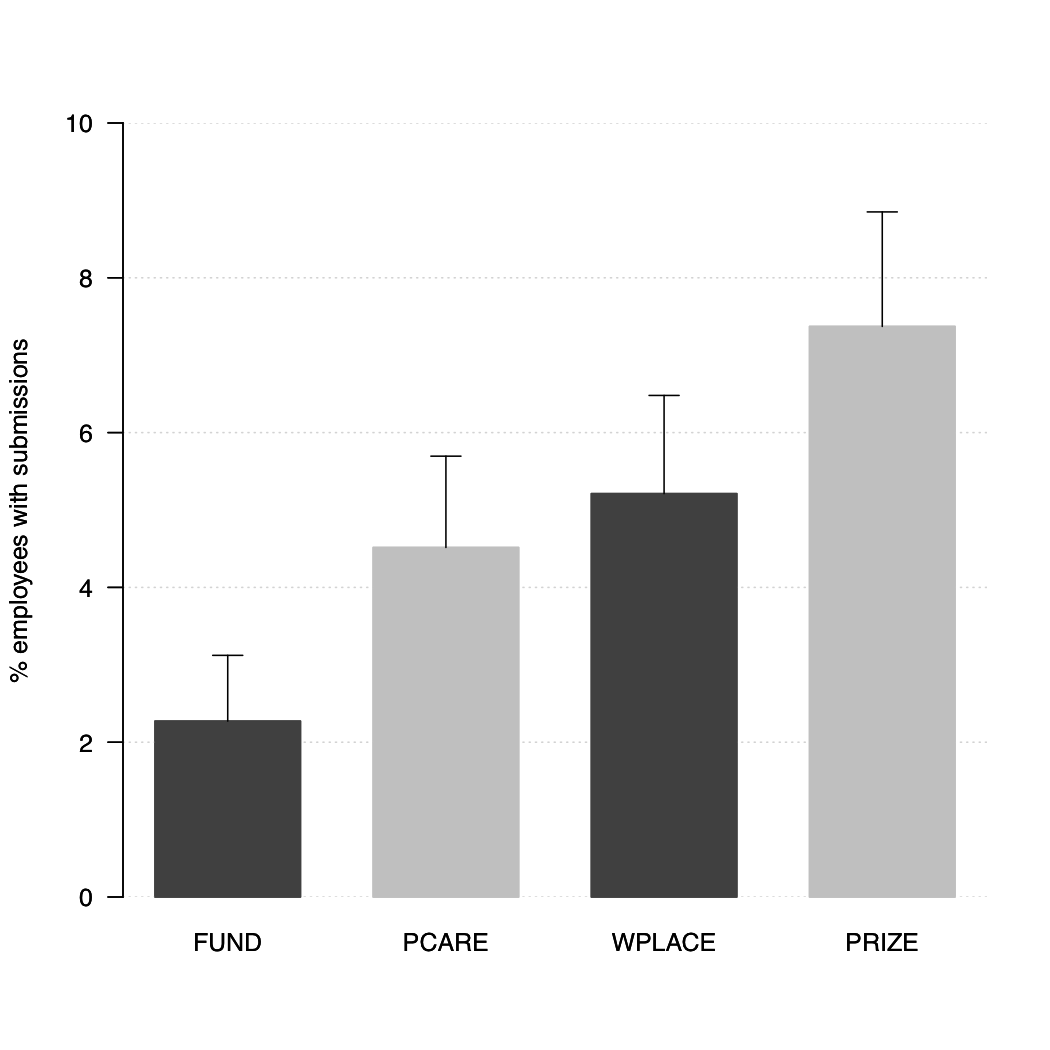
\includegraphics{../figs/part.bar.pdf}
\begin{tablenotes}
Submission rates for employees randomly assigned to different solicitation treatments (bars represent standard errors).
\end{tablenotes}
\end{figure}

Employees' submission rates range from 2 to 7 percent (Figure
\ref{fig: submit}) showing substantial variation across the randomly
assigned solicitation treatments. A Fisher's Exact Test for Count Data
indicates a statistically significant (p=0.026) association between
submission rates and solicitations, which means that the observed
variation in submission rates is, at least in part, attributable to our
experimental intervention.

Pairwise comparisons among individual solicitation treatments further
reveal that: (\emph{i}) employees in the PRIZE solicitation treatment
have 1.4, 1.6, and 3.2 times higher participation rates than those in
the WPLACE, PCARE, and FUND solicitation treatments, respectively;
(\emph{ii}) employees in the PCARE and WPLACE solicitation treatments
have basically identical participation rates; and (\emph{iii}) employees
in the FUND solicitation treatment have less than half of the
participation rates of the WPLACE and PCARE solicitation treatments.

\begin{table}
\centering
\caption{P-values for pairwise comparison of proportions}
\label{pairwise}
\begin{tabular}{@{}lccc}
  \\[-1.8ex]\hline \hline \\[-1.8ex]
 & FUND & PCARE & WPLACE \\ 
  \hline \\[-1.86ex]
PCARE & 0.124 &  &  \\ 
  WPLACE & 0.055 & 0.688 &  \\ 
  PRIZE & 0.003 & 0.132 & 0.269 \\ 
   \\[-1.8ex]\hline \hline \\[-1.8ex]
\end{tabular}
\begin{minipage}{\textwidth}\itshape\footnotesize
Note: This table reports the p-values of pairwise comparisons of proportions
						         among solicitation treatments.
\end{minipage}
\end{table}


To test to see whether these pairwise differences are statistically
significant, we use Pairwise comparison of proportions (Table
\ref{pairwise}). The analysis reveals that: a significant positive
difference in participation rates between the PRIZE and FUND
solicitation treatments (p=0.003); a marginally significant positive
difference between the PRIZE and PCARE solicitation treatments
(p=0.132); and an insignificant positive difference between the PRIZE
and WPLACE solicitation treatments (p=0.269); a significant negative
difference between the FUND and WPLACE solicitation treatments
(p=0.055); and a marginally significant negative difference between the
FUND and the PCARE solicitation treatments (p=0.124). Overall, these
findings are consistent with employee participation being higher under a
solicitation with personal awards incentives; and lower under a
solicitation with funding incentives.

A multiple linear regression model that explicitly controls for
observable differences across staff members serves to complement the
above univariate analysis. Let \(Y_i=1\) denote employee \(i\) making a
submission, and \(Y_i=0\) otherwise. We assume the conditional
probability of an employee making a submission is given by:

\[\Pr(Y_i=1) = \alpha_0 
                                    + \sum_{j} \alpha_{j} \text{SOLICIT}_{ij}
                                    + \text{JOB}_{i} 
                                    + \text{MALE}_{i} 
                                    + \text{OFFICE}_{i},\label{eq: submit}\]

where \(\alpha_0\) is a constant, \(\alpha_j\) is the causal effect of
the solicitation treatment \(j\) assigned to an employee \(i\)
(\(\text{SOLICIT}_{ij}\)), controlling for the employee's profession
(\(\text{JOB}_i\)), the gender (\(\text{MALE}_i\)), and a dummy for
office location (\(\text{OFFICE}_i\)) indicating whether the employee
had a permanent office instead of being assigned to a ward. As discussed
before, in our context, having a fixed office location is highly
correlated with the type of profession. Within each profession, however,
having a fixed office location is usually correlated with the experience
or hierarchical position inside the organization. Hence, more than just
the effect of having a fixed office location per se, this variable is
potentially controlling for income and hierarchical differences
occurring within each profession.

\begin{table}
\centering
\caption{Probability of submitting proposals}\label{participation ols}
\begin{tabular}{@{\extracolsep{5pt}}lccccc} 
\\[-1.8ex]\hline 
\hline \\[-1.8ex] 
 & \multicolumn{5}{c}{\textit{Dependent variable:}} \\ 
\cline{2-6} 
\\[-1.8ex] & \multicolumn{5}{c}{ $SUBMIT_{ij}=1$ } \\ 
\\[-1.8ex] & (1) & (2) & (3) & (4) & (5)\\ 
\hline \\[-1.8ex] 
 PRIZE & 2.53$^{**}$ & 2.53$^{**}$ & 2.52$^{**}$ & 2.46$^{**}$ & 2.45$^{**}$ \\ 
  & (1.21) & (1.21) & (1.21) & (1.21) & (1.21) \\ 
  & & & & & \\ 
 WPLACE & 0.37 & 0.37 & 0.35 & 0.38 & 0.30 \\ 
  & (1.09) & (1.09) & (1.10) & (1.09) & (1.10) \\ 
  & & & & & \\ 
 FUND & $-$2.57$^{***}$ & $-$2.57$^{***}$ & $-$2.55$^{***}$ & $-$2.49$^{***}$ & $-$2.38$^{***}$ \\ 
  & (0.86) & (0.86) & (0.85) & (0.86) & (0.85) \\ 
  & & & & & \\ 
 Job (nursing) &  & 0.14 &  &  & 1.85 \\ 
  &  & (0.82) &  &  & (1.23) \\ 
  & & & & & \\ 
 Job (MD) &  & $-$0.31 &  &  & $-$1.14 \\ 
  &  & (1.03) &  &  & (1.24) \\ 
  & & & & & \\ 
 Male (yes) &  &  & $-$0.54 &  & $-$0.42 \\ 
  &  &  & (1.33) &  & (1.64) \\ 
  & & & & & \\ 
 Office (yes) &  &  &  & 2.79$^{**}$ & 4.56$^{***}$ \\ 
  &  &  &  & (1.20) & (1.60) \\ 
  & & & & & \\ 
 Constant & 4.84$^{***}$ & 4.78$^{***}$ & 5.00$^{***}$ & 3.35$^{***}$ & 1.97 \\ 
  & (0.61) & (0.66) & (0.73) & (0.75) & (1.25) \\ 
  & & & & & \\ 
\hline \\[-1.8ex] 
Log Likelihood & -5545 & -5545 & -5545 & -5542 & -5540 \\ 
Observations & 1,237 & 1,237 & 1,237 & 1,237 & 1,237 \\ 
\hline 
\hline \\[-1.8ex] 
\end{tabular} 
\begin{minipage}{\textwidth}
\emph{Note:} This table reports OLS estimates with heteroskedasticity robust standard errors in parenthesis. All coefficients are multiplied by 100 to indicate a percentage point change in the probability of submitting. Solicitation treatment dummies are coded to indicate deviations from the overall probability of submitting. The asterisks $^{\ast\ast\ast}$, $^{\ast\ast}$, $^{\ast}$ indicate significance at 1, 5 and 10 percent level, respectively.
\end{minipage}
\end{table}


We report the OLS estimated coefficients for the above model (Table
\ref{participation ols}) expressed as solicitation treatment differences
relative to the overall mean participation. Results are consistent with
what discussed before. At the 95 level of statistical significance,
employees in the PRIZE solicitation treatment are about 2 percentage
points \emph{more} likely to submit compared to the overall mean,
whereas employees in the FUND solicitation treatment are 2 percentage
points \emph{less} likely to do so. Although these effects might appear
small in absolute terms, they are fairly large in comparison to the
overall participation rate (5 percent).

\begin{figure}
\caption{Sorting}
\label{fig: sorting}
\includegraphics{../figs/sorting.bar.pdf}
\begin{tablenotes}
Submission rates by the gender, job, and office status of the solicited employees (bars represent standard errors).
\end{tablenotes}
\end{figure}

\subsubsection{Sorting}\label{sorting}

We now look at how the willingness to participate in the contest is
associated with relevant individual characteristics, like the gender,
profession, and status inside the organization of the solicited worker.
Following the literature on gender-based differences in preferences
\citep{croson2009gender} --- like attitudes towards competitive settings
\citep{niederle2007women} --- one may expect gender to be a factor
driving participation in the contest, with men relatively more willing
to sort into the competition. Contrary to these expectations, the
submission rate for women (Figure \ref{fig: sorting}) appears higher
than that for men and testing the difference in a regression with
controls (as in the last column of Table \ref{participation ols}) gives
insignificant results (p=0.689). Similarly, one may expect the presence
of effects associated with differences in income and education as
captured by the profession of the solicited employee. Consistently with
this view, physicians appear to have a lower propensity to submit
(Figure \ref{fig: sorting}) relative to the other workers, whereas it
appears higher for nurses, but testing them in a regression with
controls gives again insignificant results (p=0.989). Finally, and
somewhat surprisingly, we find that having an office location, as
opposed to being assigned to a ward, is significantly (p=0.003)
associated with a higher submission rate, controlling for the other
characteristics. This evidence is suggesting that workers who occupy
higher positions inside the organization are also more willing to
contribute to common goods. Hence, and overall, we find no evidence
supporting sorting based on the gender and profession of the solicited
employee, whereas we find evidence for sorting based on having an office
location, which we interpret as a proxy for experience and status inside
the organization.

\begin{figure}
\caption{Submission time dynamics}
\label{dynamics}
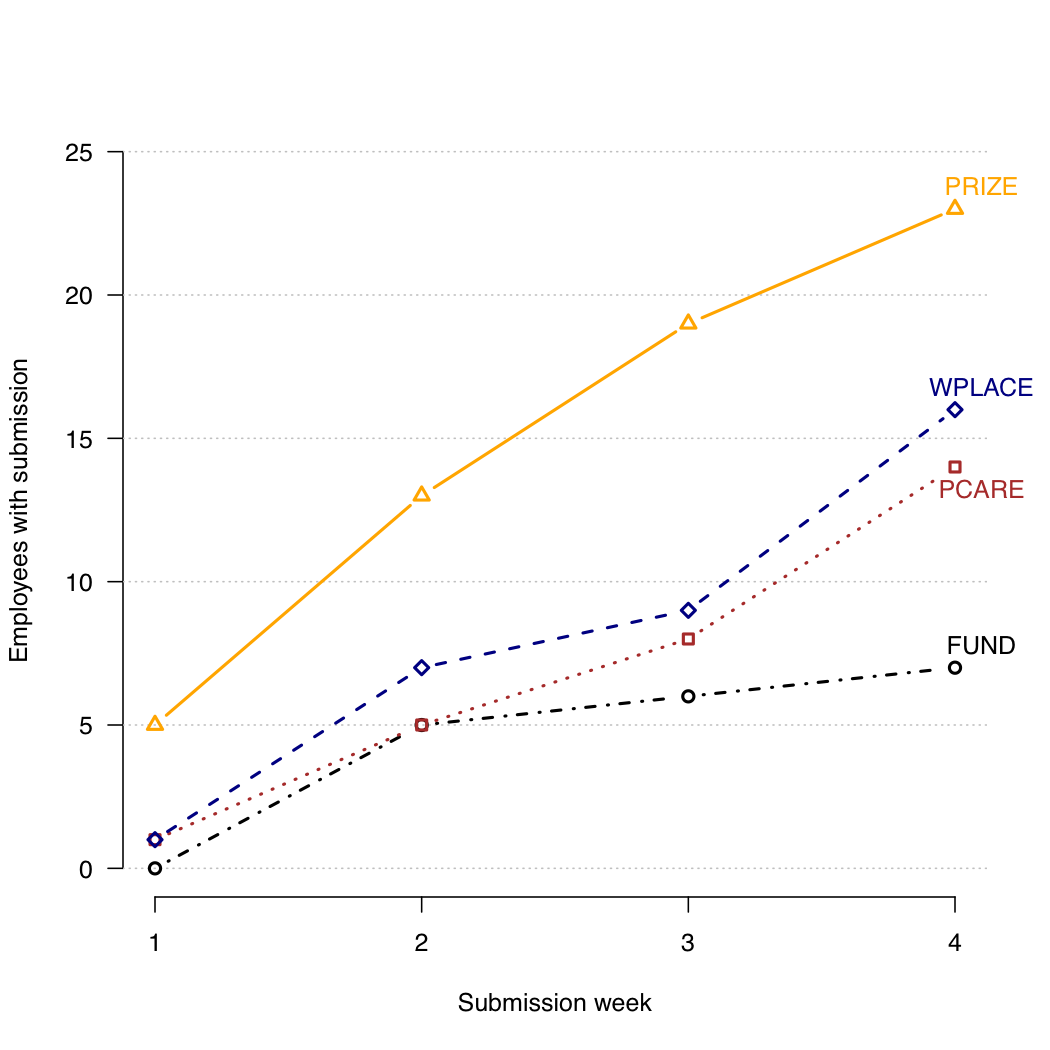
\includegraphics{../figs/dynamics.pdf}
\begin{tablenotes}
The plot shows the evolution of the cumulative sum of submissions by solicitation treatment. Employee participation in the PRIZE treatment is higher than the other solicitation treatments at all periods. By contrast, employee participation in the FUND treatment is lower at all periods. The plot also shows little convergence of the participation rates over time.
\end{tablenotes}
\end{figure}

\subsubsection{Participation dynamics}\label{participation-dynamics}

We now turn to examining participation dynamics (Figure \ref{dynamics}).
Though our data may not allow for a complete analysis of participation
dynamics, looking at the overall submission patterns can be useful for
the following reason. If employees assigned to different solicitation
treatments were sharing (either face-to-face or electronically) the
content of their solicitation with others, one should expect
participation rates to converge over time, yielding estimates of the
causal effects of a solicitation treatment biased towards zero. Contrary
to these expectations, we find no evidence of convergence. Submissions
in the PRIZE solicitation treatment are constantly higher than in the
other treatments (except perhaps in the final week); at the same time,
submissions in the FUND treatment are constantly low. These patterns are
hence consistent with communication effects having little, or no,
consequences on our findings, a topic we will discuss in greater detail
later.

\begin{figure} 
\caption{Employee participation by gender or profession and solicitation treatment}
  \label{interactions}
  \centering
  
\includegraphics{../figs/interactions.pdf}
\begin{tablenotes}
Panel (a) shows the proportion of submissions conditional on the gender of the solicited employee. Women seem more likely (about 5 percentage points) to participate than men in the PCARE solicitation treatment. Panel (b) shows the same proportion conditional on the profession of the solicited employee. Physicians, who are the highest paid professionals in our setting, are as likely to submit as any other worker in PRIZE solicitation treatment; thus suggesting little sorting based on income or other characteristics associated with a given profession.
\end{tablenotes}
\end{figure}

\subsubsection{Heterogeneous treatment
effects}\label{heterogeneous-treatment-effects}

Inspection of the participation rates conditional to the employee's
gender or profession (Figure \ref{interactions}) suggests relevant
treatment interactions based on the gender.\footnote{We find no
  significant differences for interactions with office location, which
  we do not report for space limitation.} Gender interactions may occur
as a result of three main factors: differences in risk taking, social
preferences (willingness to contribute to public goods), and competitive
inclinations. If women prefer to work on activities that are less risky,
more pro-social (e.g., aiming at improving people's health) and where
competition is less intense, then we should observe significant
treatment interactions. Similarly, one may expect treatment interactions
associated with the employee's profession to occur because, for example,
the prize opportunity could be relatively less effective for employees
with a higher income, such as doctors.

\begin{table}
\centering
\caption{Gender differences}\label{tab: probability submitting interactions}
\begin{tabular}{@{\extracolsep{5pt}}lccc} 
\\[-1.8ex]\hline 
\hline \\[-1.8ex] 
 & \multicolumn{3}{c}{\textit{Dependent variable:}} \\ 
\cline{2-4} 
\\[-1.8ex] & \multicolumn{3}{c}{ $SUBMIT_{ij}=1$ } \\ 
\\[-1.8ex] & (1) & (2) & (3)\\ 
\hline \\[-1.8ex] 
 PRIZE$\times$female & 2.99$^{*}$ & 2.95$^{*}$ & 2.84 \\ 
  & (1.68) & (1.79) & (1.78) \\ 
  & & & \\ 
 PCARE$\times$female & 1.25 & 1.21 & 1.08 \\ 
  & (1.57) & (1.61) & (1.61) \\ 
  & & & \\ 
 FUND$\times$female & $-$2.91$^{***}$ & $-$2.95$^{**}$ & $-$2.79$^{**}$ \\ 
  & (1.06) & (1.20) & (1.19) \\ 
  & & & \\ 
 WPLACE$\times$female & $-$0.49 & $-$0.52 & $-$0.62 \\ 
  & (1.35) & (1.44) & (1.43) \\ 
  & & & \\ 
 PRIZE$\times$male & 1.37 & 1.42 & 1.40 \\ 
  & (2.44) & (2.51) & (2.50) \\ 
  & & & \\ 
 PCARE$\times$male & $-$3.75$^{***}$ & $-$3.72$^{***}$ & $-$3.64$^{***}$ \\ 
  & (1.15) & (1.16) & (1.16) \\ 
  & & & \\ 
 FUND$\times$male & $-$1.67 & $-$1.65 & $-$1.48 \\ 
  & (1.70) & (1.65) & (1.66) \\ 
  & & & \\ 
 Constant & 4.80$^{***}$ & 4.79$^{***}$ & 1.87$^{*}$ \\ 
  & (0.69) & (0.70) & (1.10) \\ 
  & & & \\ 
\hline \\[-1.8ex] 
Job & no & yes & yes \\ 
Office & no & no & yes \\ 
Log Likelihood & -5542 & -5542 & -5538 \\ 
Observations & 1,237 & 1,237 & 1,237 \\ 
\hline 
\hline \\[-1.8ex] 
\end{tabular} 
\begin{minipage}{\textwidth}
\emph{Note:} This table reports OLS estimates with heteroskedasticity robust standard errors in parenthesis. All coefficients are multiplied by 100 to indicate the percentage point change in the probability of submitting. Solicitation treatment dummies are coded to indicate deviations from the overall probability of submitting. The asterisks $^{\ast\ast\ast}$, $^{\ast\ast}$, $^{\ast}$ indicate significance at 1, 5 and 10 percent level, respectively.
\end{minipage}
\end{table}


To isolate gender and profession effects, we employ a version of model
\eqref{eq: submit} with gender-treatment interactions. The regression
results (Table \ref{tab: probability submitting interactions}) show
similar results to the simple comparison of proportions. That is, after
gradually adding profession and office controls, interaction
coefficients remain stable across all specifications: the response of
men under the PCARE solicitation treatment is about 3 times the
magnitude and in the opposite direction of the women's response. By
subtracting these two coefficients, we find a significant difference
between men and women of about 5 percentage points (\(p=.018\)), which
is consistent with our previous analysis. Thus, and overall, men respond
less than women in the PCARE solicitation treatment, controlling for the
profession and office location. This effect could be due to gender
differences in preferences, as suggested by the literature, and we will
return on this topic in the discussion of the results.

\subsection{Employee participation in peer
evaluation}\label{employee-participation-in-peer-evaluation}

We now turn to examining the outcomes of the peer evaluation that
follows the submission period. In this phase, 113 project proposals
ended up being rated by a total of 178 employees (14 percent of our
sample) who volunteered for the task. Their effort yielded a total of
12,219 evaluator-proposal pairs, providing a very sensitive test for
differences in project quality across our solicitation treatments.

\input{../tables/ratings_by_treatment.tex}

We note (Table \ref{ratings}) that employees who are in the PCARE and
WPLACE solicitation treatments seem to have a higher propensity to
evaluate proposals than those in the PRIZE and FUND solicitation
treatments. Since evaluating proposals is another way for workers to
contribute to the organization, workers will have incentives similar to
those in the submission phase so that indirect treatment effects are
plausible. However, no evidence is found that the observed differences
in evaluation rates are attributable to our experimental intervention (a
Fisher's exact test gives a p-value of 0.339). In other words, our data
do not seem to support the hypothesis of treatment effects on evaluating
proposals.

We further check for sorting to see whether the evaluators are wholly
representative of the organization. Testing for the statistical
significance of coefficients for the profession, gender, and office
location in a linear regression on the probability of evaluating
proposals (results not shown), we find no differences based on the
employee's gender and profession albeit a significantly higher
participation from staff members with an office location. This evidence
is thus consistent with our previous results about participation in the
submission phase; suggesting the collected assessments of proposal
quality are made by a broadly representative sampling of opinions inside
the organization.

\subsection{Quality of the project
proposals}\label{quality-of-the-project-proposals}

The treatment interventions may not have only impacted the propensity to
make a submission, but the quality of the submission as well. Of
particular interest is any indication of a quantity versus quality
trade-off. For example, if the treatment which generated the fewest
submissions (FUND) also produced the highest quality submissions. A
quality versus quantity trade-off would increase the complexity of
choosing optimal incentives for employees. We examine the issue with the
assessments of quality made by peers in the evaluation phase of the
contest and, subsequently, by the management.

\subsubsection{Quality assessed by
peers}\label{quality-assessed-by-peers}

To check whether differences in the quality of the submissions can be
explained by the solicitation treatments of the submitter, we first look
at differences in the distribution of ratings obtained from peers.
Overall, a project proposal is given the ``neutral'' point (i.e., a
rating of 3) on a five-point scale about 30 percent of the times with
employees being more likely to give high (4-5) rather than low (1-2)
ratings. This pattern does not change much when we condition the data to
the solicitation treatment of the proponent (Figure \ref{fig: quality});
suggesting an equal distribution of good and bad quality projects across
the solicitation treatments.

\begin{figure}
\centering
\caption{Differences in the quality of the submitted project proposals}
\label{fig: quality}
\includegraphics{../figs/quality.pdf}
\end{figure}

To formally test this hypothesis, we aggregate mean ratings for each
proposal and regress these aggregate measures on solicitation treatment
dummies. The regression results (not reported) show only an
insignificant relationship between ratings and solicitation treatments.
The treatment coefficients are all insignificantly different from zero,
with the linear model not significantly different from a constant model
(an overall F-test gives a p-value of 0.609).

We also examine the distribution of ratings as generated by treatments
with no aggregation.\footnote{The analysis on the aggregated data
  crucially relies on the assumption that an increment in a proposal's
  quality as measured by an increase in ratings from \(v\) to \(v+1\) is
  the same for any value \(v\).} We have over 12,000 ratings, providing
a very sensitive test for differences across treatments. Using a
Pearson's Chi-squared test we find that the hypothesis of dependence
between the distribution of ratings and the treatments is \emph{not}
quite significant at the 10 percent level (p-value of 0.103). Driving
the p-value is a less than \(2\) percent difference between the
proportion of 5's in the WPLACE treatment versus the other
distributions, which is probably due to outliers (the winning proposal
was in the WPLACE treatment). Taken together with the fact that our
sample is large, we have strong evidence suggesting that there are no
(economically meaningful) differences in the quality of project
proposals across treatments and in particular no evidence of a quantity
versus quality trade-off up to the resolution of the five-point
scale.\footnote{One may worry that such binning is a fairly coarse
  measure of quality. In particular, effects concentrated in the upper
  tail of the distribution may not be detected. For example, comparing
  the ratings of proposals A, B, C and D with hypothetical true
  qualities of 3, 4, 5, and 10 stars respectively. Under a five-point
  scale rating system, proposals A and B can be distinguished, but C and
  D cannot be distinguished. Hence, one needs to be very cautious in
  interpreting these results as evidence against quality effects in
  general.}

\subsubsection{Quality assessed by
managers}\label{quality-assessed-by-managers}

One potential limit of assessing quality only on the basis of peer
ratings is that the employees might have a different view of a
proposal's quality than executives (due, for instance, to a misalignment
of incentives). Indeed, to ensure alignment between managerial goals and
the peer assessment, all project proposals were further vetted by the
HTL staff before being considered for implementation funding. We now
focus on the outcomes of this vetting process to investigate more
broadly the presence of treatment effects on the quality of project
proposals.

The vetting process conducted by the HTL staff resulted in 93 proposals
being scored on a scale from 1 to 100 points with the authors of the
best 29 proposals being invited to submit implementation plans. The
remaining 20 proposals were excluded (and received a score of zero)
either because flagged as inappropriate for funding or because the
proponent manifested no intention to participate in the implementation
phase (we find no association between proposals excluded and
treatments).

As a broad measure of agreement between peer ratings and the assessment
made by the management we use the Spearman's rank correlation
coefficient between the scores given by the HTL staff and the average
peer ratings. Results show a relatively high correlation (cor=0.198),
indicating good agreement between our two measures of quality. As for
the assessments made by peers, using the scores by the management shows
no treatment effects on quality: a linear regression on the score of
proposals against treatment dummies gives coefficients that are all
insignificantly different from zero, with the linear model not
significantly different from a constant model (F-test; p=0.378).

Being selected and invited to submit additional implementation plans is
another indication of quality assessed from the management perspective.
A simple test for independence between the percentage of submitters
being selected and invited by HTL staff and the randomly assigned
solicitation treatment gives no significant results (a Fisher's Exact
Test for Count Data gives a p-value of 0.253). Although not significant,
employees who made project proposals in the FUND solicitation treatment
are \emph{less} likely to be selected as finalist than the others (only
1 out of 7 in the FUND treatment were selected and invited by the HTL
staff), providing additional evidence of a no quantity versus quality
trade-off, as discussed before.

\subsubsection{Quality assessed by higher word
counts}\label{quality-assessed-by-higher-word-counts}

Following prior research indicating that higher total word counts
reflect higher quality \citep{blumenstock2008size}, we also look at
differences in the word counts of a submission. We find that most
submissions are below 200 words with little differences between the
treatments. Testing for a significant linear regression relationship
between the length of submissions and treatment dummies returned an
overall insignificant result (p=.43, F-test), which is consistent with
our previous assertion of little, or no, differences in quality across
treatments.

\subsection{Content of the project
proposals}\label{content-of-the-project-proposals}

While we have shown little differences in the overall project quality
across solicitation treatments, it is easy to think of ways in which a
solicitation may affect the \emph{content} of the submitted proposals,
while keeping the quality constant. For example, different solicitations
may lead proponents to think about different kinds of problems or,
indirectly, through the sorting of proponents with differing needs or
knowledge of the problems inside the organization.

Before examining specific differences in the content of proposals, it is
important to point out that the proposed projects broadly conformed to
the stated goals of the contest, which was to improve Heart Center
operations by identifying problem areas and potential solutions. For
example, one project proposal that received high peer ratings was to
create a platform for patients to electronically review and update their
medicine list in the office prior to seeing the physician. Another was
to develop a smartphone application showing a patient's itinerary for
the day providing a guide from one test or appointment to another. This
suggests the aligning with improving the work processes within the
organization or providing high-quality patient care. Nevertheless, other
contest organizers may have varying goals and be concerned about
different aspects of the submissions.

To examine additional dimensions of submission content, we now study the
\emph{area of focus} of the submissions. Of particular interest is
understanding whether different wordings used in the general
encouragement solicitation (either towards improving the workplace or
targeting the wellbeing of patients) induce employees to concentrate on
different categories of interventions. Members of the HTL categorized
each project proposal into one of seven areas of focus (Table
\ref{tab: area-of-focus}): three categories (``Care coordination'',
``Staff workflow'', ``Workplace'') identified improvements for the
workplace, other three (``Information and access'', ``Patient care'',
and ``Quality and Safety'') focused on improvements centered around
patients, and another one (``Surgical tools and support to research'')
categorized projects developing tools to support scientific research.

\begin{figure}
\caption{Differences in the content of the submitted project proposals}
\label{fig: content}
\includegraphics{../figs/areas.pdf}
\begin{tablenotes}
The four panels show the proportions of submitted project proposals in each area of focus (a=Surgical tools and support to research,b=Quality and safety ,c=Workplace,d=Staff workflow,e=Care Coordination,f=Information and access,g=Patient support) for each solicitation treatment. The proportions of the WPLACE treatment are used as a reference in all panels.
\end{tablenotes}
\end{figure}

The proportions of submitted project proposals in each area of focus
(Figure \ref{fig: content}) exhibit very similar patterns for the WPLACE
and PRIZE solicitation treatments and different and uncorrelated
patterns for the other treatments; suggesting the presence of treatment
effects. We test to determine the overall association between these
proportions and our solicitation treatments with a Fisher's Exact Test
for Count Data with simulated p-value (based on 50000 replicates).
Results show a significant (p=0.088) association at the 90 percent
level, providing thus evidence that the variation in the content of the
submitted proposals is, at least in part, attributable to our
experimental solicitations.

To test which areas of focus is affected by our treatment, we regress
the probability of a project proposal being in a given category against
solicitation treatment dummies. We use an F-test where the null
hypothesis tested is that all the treatment effects have a zero effect
on the probability of the proposal being in a given category. The
results show that project proposals in the PCARE solicitation treatment
are less likely to fall in the ``Quality and Safety'' category; and
project proposals in the FUND solicitation treatment are less likely to
fall in the ``Information and access'' category.

Although it is difficult to interpret these results because our model
does not provide any prediction on the content of proposals, they
indicate a possible trade-off between stimulating participation via
solicitation and inducing selection in the type of contributions to the
public good, which complicates the analysis of incentives for public
goods inside organizations beyond what the current literature
anticipates.

\subsection{Estimating social
preferences}\label{estimating-social-preferences}

The analysis above has shown that our solicitation treatments had both
positive and negative effect on participation, with no effects on
quality. But what can we say about the employees' preferences towards
the common goal of improving the organization?

To gauge the magnitude of underlying preferences for contributing to the
organization, we now use the experimental data to calibrate the
theoretical model discussed before (Section
\ref{conceptual-framework-and-predictions}). Following the
mixed-strategy equilibrium of the model, the theoretical probability of
contributing must be proportional to the expected value of winning,
\(R\), the underlying preferences towards the public good, \(\gamma\),
the marginal costs of contributing, \(c\), and the number of agents,
\(n\).

We assume the cost of making a submission \(c\) is the same in each
treatment, which seems a reasonable assumption given everyone is asked
to perform the exact same task (submitting a project proposal) and the
submission procedure is identical. Then we derive a structural
relationship between the observed difference in the probability of
contributing \(\Delta p\) and the difference in the expected rewards
from winning \(\Delta R\) between the treatments:\footnote{This equation
  can be obtained by following these steps. First, we approximate the
  profit equating condition \eqref{eq: mixed-strategy} to a linear
  function by noticing that the \(1/(1-(1-p)^n)\) approximates one for
  \(n\) large enough and \(p\) sufficiently small. Second, we solve for
  \(p\) and we simplify using the definitions of \(\Delta p\) and
  \(\Delta R\).}

\begin{equation}
  \label{eq: delta}
  \Delta p \approx\frac{\Delta R}{n (c - \gamma)}.
\end{equation}

(Throughout this section we will consider \(\delta=0\) ignoring the
distinction between impure and pure altruism.) By solving for the net
cost of contributing \(\Delta c=c-\gamma\), we get

\begin{equation}
  \label{eq: gamma}
  \Delta c\approx  \Delta R / (n\Delta p). 
\end{equation}

This implies that the net cost of a submission (the material cost of
submitting net of the individual preference for the public good) must be
proportional to the ratio between the difference in rewards and the
difference in the probability of submitting. Although we do not observe
the levels of \(R\) in each treatment, we approximate the difference of
rewards between the PRIZE and the other conditions by the pecuniary
value of the reward, which has its upper bound in the highest price that
can be paid for an iPad mini (\$350).\footnote{The price paid by the
  Heart Center was \$239 at the end of 2014 (including shipping cost).
  Other popular models (those with cellular data and large storage)
  could cost as high as \$350. Agents, however, were not aware of the
  specific model used for the competition and of the price paid. So, the
  value of \$350 is very conservative.} And we round the competitors up
to \(n=1000\) to be conservative. Finally, by substituting those
calibrated values into equation \eqref{eq: gamma} along with the
empirical difference in participation rates between the PRIZE and the
other treatments (\(\Delta p=0.037\)), we get an estimate of the
magnitude of net cost which is \(\Delta c=\) \$350/(1000*0.037)=\$9.5.

We can now compare the estimated net cost of contributing against the
hourly wage of the median staff member, which is \$40 (the median income
per hour of a nurse according to the Bureau of Labor Statistics). This
comparison shows that the wage of the median staff member per hour is
more than 4 times \emph{higher} than the net cost of making a
contribution. Since the time to write and submit a project proposal will
likely take one hour of work or more, the net cost of contributing
appears too low to be consistent with no preferences towards the public
good. In other words, by comparing the calibrated net cost of
contributing against the monetary cost of an hour of work, we find a
negative gap that appears too large to be explained without assuming
some non-monetary motivations acting as a compensating force.

\section{Summary and conclusions}\label{summary-and-conclusions}

We conduct a natural field experiment to better understand what makes
employees at a medical organization participate in an internal
innovation contest seeking project proposals for improving the
operations of the organization. Participation is expected to generate
positive externalities for colleagues and patients but also individual
costs thereby making free riding a salient problem.

Overall, we find a positive effect on employee participation of
solicitations offering personal rewards to the winning submissions, and
this positive effect is without changing the submission quality as
judged by peer ratings and the evaluations conducted by the management
--- for which there is good agreement (high positive correlation)
suggesting incentives being sufficiently aligned. This means that the
higher propensity to participate does not seem to be driven by
low-quality submissions. In addition, we provide evidence that the
effect on participation goes beyond the actual value of the prize
itself, thus suggesting employees have internalized some of the public
good effects of contributing. Our results also suggest that the
opportunity of funding own projects is a poor incentive. It leads to a
lower propensity to submit project proposals, and this lower propensity
does not seem to be driven by compensating effects in terms of more
high-quality submissions (if anything, average quality is lower).
Finally, solicitations appealing to altruistic motivations towards
providing better care to their patients and improving the workplace
environment, have equally strong participation propensity on average,
but we find that responses appear sensitive to the gender of the
solicited person. Women's participation is greater when emphasizing the
patient care whereas men's participation is significantly lower,
controlling for the profession and position inside the organization.
This finding suggests that gender may be an important factor influencing
sensitivity of responses to solicitations concerning the organizational
mission. At the same time, only an insignificant gender-based
differences with respect to participation associated with the offering
of prizes was found: women's participation was slightly higher but not
significant than men's, all else being equal. This evidence indicates
that gender differences in preferences, such as competitive inclinations
or risk aversion, may not exert great influence on responses of workers
to contests inside organizations.

We believe these results have three main implications for comparable
organizations and, more broadly, the internal provision of public goods.

The first implication is that announcing a competition for an individual
prize foster workers' participation in organizational tasks beyond the
value of the awarded prize itself. That is, prizes generate two opposing
externalities that help workers internalize the public good effects of
their organizational contributions. This result is important because it
highlights a relatively less understood function of contests that is to
mitigate the free riding incentives on organizational tasks.

A second implication is that offering the opportunity to lead collective
projects can exacerbate the free riding incentives. This result may
appear contrary to intuition. In theory, one may benefit more from
leading a project than winning an iPad. For instance, one may use the
opportunity to signal project management skills to the management aiming
for a career advancement; or steer some of the resources towards assets
or problems that are relatively more beneficial to his or her situation
compared to the rest of the organization. If so, why a negative result?
We believe that the private benefits from winning were negligible in our
setting. First, the opportunity for a career advancement is small
because medical staff gets promoted on the basis of other parameters
(e.g., the quality of care provided). Second, the peer evaluation and
vetting by the management ensure that the winning contributions yield as
distributed benefits as possible. These aspects may have eliminated the
possible private benefits from leading a project, resulting in poor
participation rates. This result is important because projects need to
be lead by someone and making more resources available does not seem to
increase volunteers.

A third implication is that participation in organizational tasks is
sometimes triggered by mission-based preferences. Although we find
evidence that these preferences can be an effective incentive, we also
find gender-based selection effects that are difficult to predict
ex-ante. Our experiment does not provide any insights to better
interpret these differences. But a large literature has investigated
gender-based difference in preferences \citep[see][ for a
review]{croson2009gender} or difference in self-stereotypes
\citep{coffman2014evidence} that could explain some of these effects.
Yet, more experimentation is needed to understand the different drivers
in the field inside organizations.

A few limitations of this study deserve consideration. The first is that
the validity of our causal interpretation of the results rests on a few
conventional assumptions \citep{rubin1974estimating}. These include the
``no interference between units'' assumption. In our study, it is
possible that communication among staff assigned to different treatment
arms could have influenced decisions to participate. The magnitude of
this interference would depend on intensity of staff communication and
the density of social interactions. Both of which should be small
because (i) an individual competition may provide only weak incentives
for information sharing and (ii) the staff members are scattered across
multiple buildings on the hospital campus. Even so, a potential
inference bias may alter the results towards a null effect as
differences in employee participation should converge towards zero when
communication spreads the content of the different email solicitations.
This goes against our results. Moreover, by looking at the temporal
dynamics of submissions, we find no indication of a convergence in the
participation rates. Hence, the assumption of no interference seems
appropriate.

Another potential limitation is that staff members may have left the
solicitation email that was sent to them unopened or unread, thus
non-complying with the assigned solicitation treatment. As this kind of
noncompliance is almost entirely unobserved,\footnote{The email was sent
  using the internal messaging system of the Heart Center, which, at the
  time, was not collecting individual analytics.} the analysis follows
an \emph{Intention-To-Treat} (ITT) approach, discarding entirely any
information about the solicitation treatment actually received. The main
drawback of an ITT analysis is that it does not answer questions about
causal effects of the content of the solicitation itself, only about
causal effects of the assignment to a solicitation treatment.

Finally, our results have implications that extend beyond the specific
organization under study. While the choice of focusing on health care
workers may limit the generalizability of our results in some respect,
it should be noted that in the US alone health care spending accounts
for 17 percent of the GDP (in 2015). And, more generally, our study
results are also directly applicable to a variety of other professions
exposed to a public good dilemma in a mission-driven environment (e.g.,
teachers, public servants, researchers). In all these settings, our
study suggests that contests soliciting employee contributions and
awarding an individual prize to the winning contribution appear an
effective way to foster the internal provision of public goods inside
organizations.

\renewcommand\refname{References}
\bibliography{refs.bib}

\end{document}